\documentclass{beamer}

\usepackage{subfigure}
\usepackage{graphicx}
\usepackage{sidecap}
\usepackage{caption}
%\usepackage{subcaption}
\captionsetup{compatibility=false}
\usepackage{appendixnumberbeamer}
\usepackage{amsmath}
% --
\usepackage{multirow}
\usepackage{xcolor}
\usepackage{setspace}
\usepackage{hyperref}
\usepackage{anyfontsize}

\setbeamertemplate{footline}

\newenvironment{itemise} {\begin{itemize} \setlength{\itemsep}{0.2cm}} {\end{itemize}}
\usepackage[labelformat=empty]{caption}
\setbeamertemplate{sections/subsections in toc}[square]

%% COLORS
\definecolor{Gray}{gray}{0.9}
\definecolor{dblue}{rgb}{0.132,0.1,0.27}
\definecolor{mint}{cmyk}{1.0, 0.2, 0.6, 0.05}
\definecolor{ant}{cmyk}{0.5, 0.1, 0.0, 0.45}
\definecolor{lgray}{cmyk}{0.12, 0.0, 0.0, 0.17}
\definecolor{lred}{cmyk}{0.0, 0.9, 0.7, 0.0}


\usepackage{etoolbox}% http://ctan.org/pkg/etoolbox 
\usepackage{booktabs}

\newenvironment{literatur}{%
  \parskip2pt \parindent0pt \raggedright
  \def\lititem{\hangindent=0.5cm \hangafter1}}{%
  \par\ignorespaces}

\newcommand{\tb}[1]{{\color{blue}{\textbf{#1}}}}
\newcommand{\tm}[1]{{\color{mint}{\textbf{#1}}}}
\newcommand{\tr}[1]{{\color{red}{\textbf{#1}}}}
% Ilya: packages

\usepackage{tikz}
\usepackage{lmodern}
\usepackage{enumitem}

% Ilya: my commands

\newenvironment{mytemize}
{\vfill\itemize[nolistsep,itemsep=\fill,label=\color{blue}{$\triangleright$}]}
  {\enditemize}


\newenvironment{mynumerate}
{\vfill\enumerate[nolistsep,itemsep=\fill,label=\arabic*.]}
  {\endenumerate}

\newcommand{\hitem}[1]{
  {\color{blue}{$\triangleright$}} 
  {#1} 
  {\hfill}
}

\setlist[itemize]{label= \color{blue}{$\triangleright$}}
\setlist[enumerate]{label = \arabic*.}

\newcommand{\rarr}{$\Rightarrow$\ }



%\href{<Ziel>}{<Eingefasster Text>} 

%\logo{\includegraphics[height=0.7cm]{BdFlogo.eps}\hspace{300pt}\vspace{-5pt}}
%\logo{\includegraphics[height=0.8cm]{BdFlogo.eps}}
%\logo{\pgfputat{\pgfxy(-6.2,-0.5)}{\pgfbox[center,base]{\includegraphics[height=0.8cm]{BdFlogo.eps}}}}

%------------------------------------------------------------------------------------
% TITLE
%------------------------------------------------------------------------------------
\title[PSME]{Macroeconomics\\ Lecture 6 -- Real Business Cycles} 
\author[I. Eryzhenskiy]{Ilya Eryzhenskiy}
\institute[BdF]{PSME Panth\'{e}on-Sorbonne Master in Economics}
\date[PSME macro]{Fall 2022}

%---BEGIN------------------------------------------------------------------------------
\begin{document}

\begin{frame}
  \maketitle
\end{frame}

\begin{frame}{Overview}
  \tableofcontents
\end{frame}


\section{Model specification}
\subsection{Households}

\begin{frame}{Consumer optimization}

{
Lagrangian of consumer problem
\begin{align*}
\mathcal{L} = E_0 \sum_{t=0}^{\infty} \beta^t 
\{  &u(C_t,1-L_t) \\
&+ \lambda_t \left[ w_t L_t + (1+r_t) \Omega_t + \Pi_t -C_t - \Omega_{t+1}\right] \}
\end{align*}
Budget constraint holds as equality for all $t$ \rarr $\lambda_t > 0$ for all $t$.
First-order conditions in period $t$:
\begin{align*}
&(1) \quad \frac{\partial \mathcal{L}}{\partial C_t} \quad &  &u'_c(C_t,1-L_t)-\lambda_t = 0\\
&(2) \quad \frac{\partial \mathcal{L}}{\partial L_t} : \quad &  &u'_{1-L}(C_t,1-L_t)+ \lambda_t w_t=0\\
&(3) \quad \frac{\partial \mathcal{L}}{\partial \Omega_{t+1}} : \quad &  &-\lambda_t +\beta E_t[\lambda_{t+1}(1+r_{t+1})]=0 
\end{align*}
}
\tb{$\lambda_t = u'_c(C_t, 1-L_t)$} follows from (1): $\lambda_t$ is marginal utility of consumption at $t$, also known as \tb{shadow price} of wealth. 

\end{frame}
%---FRAME------------------------------------------------------------------------------
\begin{frame}{Labour supply}

\begin{mytemize}
\item Eliminate $\lambda_t$ from FOC (1), (2) to get the \tm{consumption-labor optimality condition}:
\begin{align*}
\frac{u'_{1-L}(C_t,1-L_t)}{u'_c(C_t,1-L_t)}= w_t
\end{align*}
\item defines (implicity) the function of \tm{labour supply for a given level of consumption}
\begin{align*}
L_t = L^s(w_t, C_t)
\end{align*}
\item features substitution and income effects: sign of $w_t$ derivative is ambiguous
\item number (or share) of hours worked is the \textit{intensive margin} of labor supply. We do not have the \textit{extensive margin} (work vs. unemployment) in this model. If interested, look at Ch. 10 of Romer textbook.%``Equilibrium Unemployment Theory'' textbook of Pissarides, Nobel winner of  2010.
\end{mytemize}

\end{frame}
%---FRAME------------------------------------------------------------------------------
\begin{frame}{Consumption-savings: the Euler equation}

\begin{mytemize}
\item \tb{(1) and (3)} imply the \tm{consumption-savings optimality condition}
\begin{align*}
1 = E_t \left[ \left( \frac{\beta \lambda_{t+1}}{\lambda_t}\right)(1+r_{t+1})\right]
\end{align*}
\item \tb{Euler equation}: key equation in modern macro models
\item In finance, $E_t \frac{\lambda_{t+1}}{\lambda_t}$ known as \textbf{pricing kernel} or \textbf{stochastic discount factor}
\begin{mytemize}
\item important for finance theory $+$ studied empirically
\end{mytemize}
\item Pricing kernel, Euler equation $\rightarrow$ intersection of macro and finance theory
\end{mytemize}

\end{frame}
%---FRAME------------------------------------------------------------------------------
\begin{frame}{Consumption-savings: the Euler equation}

  Substituting $\lambda_t$ from FOC (1) and assuming no uncertainty (for this slide):
\begin{align*}
1 =  {\left( \frac{\beta u'_c(C_{t+1},1-L_{t+1})}{u'_c(C_t,1-L_t)}\right)}(&1+r_{t+1}) \\
\\
 \Leftrightarrow \frac{u'_c(C_t,1-L_t)}{\beta u'_c(C_{t+1},1-L_{t+1})}=&1+r_{t+1}
\end{align*}
\begin{mytemize}
\item \underline{Left side:} \textbf{marginal rate of substitution} (MRS) between period $t$ and $t+1$ consumption 
\item \underline{Right side:} ratio of price of period $t$ consumption ($=1$) to price of period $t+1$ consumption $\left(=\frac{1}{1+r}\right)$
\item \underline{Interpretation:} consuming $\varepsilon$ units less ($\varepsilon \to 0$, marginal amount) in $t$ and $(1+r)\varepsilon$ units more in $t+1$ must keep utility unchanged
\end{mytemize}
\end{frame}
%---FRAME------------------------------------------------------------------------------
\begin{frame}{Euler equation with uncertainty}

  Bringing back uncertainty:

\begin{align*}
  1 = E_t \left[ {\left( \frac{\beta u'_c(C_{t+1},1-L_{t+1})}{u'_c(C_t,1-L_t)}\right)}(1+r_{t+1})\right]
\end{align*}

\begin{mytemize}
\item Utility of consuming $\varepsilon$ (very small) in period $t$...
\item ... equal to the \tr{expected} utility of marginal savings with return on them, $(1+r_{t+1})\varepsilon$, at $t+1$
\item Defines (implicitly) \tb{demand for assets} or \tb{savings supply}:
\begin{align*}
\Omega_{t+1} - \Omega_t = G(E_t r_{t+1})
\end{align*}
\end{mytemize}

\end{frame}
%---FRAME------------------------------------------------------------------------------
\begin{frame}{Household choices - Summary}

  Representative household's period $t$ optimal choices of $C_t$, $L_t$ and $\Omega_{t+1}$ characterized by consumption-labor optimality condition, consumption-savings optimality condition and flow budget constraint:
\begin{align*}
1 =& E_t \left[ \left( \frac{\beta u'_c(C_{t+1},1-L_{t+1})}{u'_c(C_t,1-L_t)}\right)(1+r_{t+1})\right] \\
 w_t=&\frac{u'_{1-L}(C_t,1-L_t)}{u'_c(C_t,1-L_t)} \\
C_t + \Omega_{t+1} =& w_t L_t + r_t \Omega_t + \Pi_t
\end{align*}
taking as given $\Omega_t$ (pre-determined), $w_t$, $r_{t}$, and $\Pi_t$ \\
These define: 
\begin{mytemize}
\item demand side of period $t$ goods market (depending on $r_t$) \rarr close to IS
\item supply side of period $t$ labour market
\item supply side of period $t$ asset/savings markets (will define \tb{capital formation})
\end{mytemize}

\end{frame}

%---FRAME------------------------------------------------------------------------------
\subsection{Representative firm}
%---FRAME------------------------------------------------------------------------------
\begin{frame}
\frametitle{Outline}
\tableofcontents[currentsubsection]
\end{frame}
%---FRAME------------------------------------------------------------------------------
\begin{frame}{Representative firm}

  A large number (a mass equal to 1) of identical firms in \tb{perfect competition} \rarr study \tb{representative firm} \\
\vfill
Firms do not make intertemporal choices. They only: 
  \begin{mynumerate}
\item rent factors of production (labour and capital) on markets
\item produce goods according to $Y_t = Z_t f(K_t, L_t)$, with $Z_t$~\tb{stochastic productivity} (same for all firms) 
\item distribute profits (null in equilibrium) to households 
  \end{mynumerate}
\vfill
No difference in model if firms live for 1 or $\infty$ periods \\
\vfill
Perfect competition \rarr firm \tb{takes prices $w_t, r_t$ as given}
\vfill
Production function $f$ has $f'_L, f'_K >0; f''_L, f''_K<0$
\vfill
\tb{Constant returns to scale} in $f$ \rarr \tb{profits null in equilibrium}.
\end{frame}
%---FRAME------------------------------------------------------------------------------
\begin{frame}{Firm profit maximization}

  Productivity $Z_t$ observed at \textbf{beginning of period $t$}. Firms then optimize period $t$ profit:
\begin{align*}
  \Pi_t &= Z_tf(K_t,L_t)-w_t L_t - (1+r_t) K_t + (1-\delta)K_t \\
		&= Z_tf(K_t,L_t)-w_t L_t - (r_t + \delta) K_t 
\end{align*}
\begin{mytemize}
\item Static maximization of profit function
\begin{align*}
  \max_{\left\{ L_t,K_t \right\}} Z_t f(K_t,L_t)-w_t L_t-(r_t+\delta) K_t
\end{align*}
\item First-order conditions
\begin{align*}
L_t: \quad \quad Z_t f_L(K_t,L_t) &= w_t \\
K_t: \quad \quad Z_t f_K(K_t,L_t) &= r_t + \delta
\end{align*}
FOCs define a downward sloping \tb{labor demand function} $L^d(w_t, Z_t)$ and \tb{capital demand function} $K^d(r_t, Z_t)$
\end{mytemize}

\end{frame}
%---FRAME------------------------------------------------------------------------------
%---FRAME------------------------------------------------------------------------------
\subsection{Equilibrium}
%---FRAME------------------------------------------------------------------------------
\begin{frame}
\frametitle{Outline}
\tableofcontents[currentsubsection]
\end{frame}
%---FRAME------------------------------------------------------------------------------
\begin{frame}{Dynamic equilibrium: diagram}
\begin{center}
%{\small
%Figure. 
%}
\vspace{-5mm}
\begin{figure}[h!]
	\subfigure{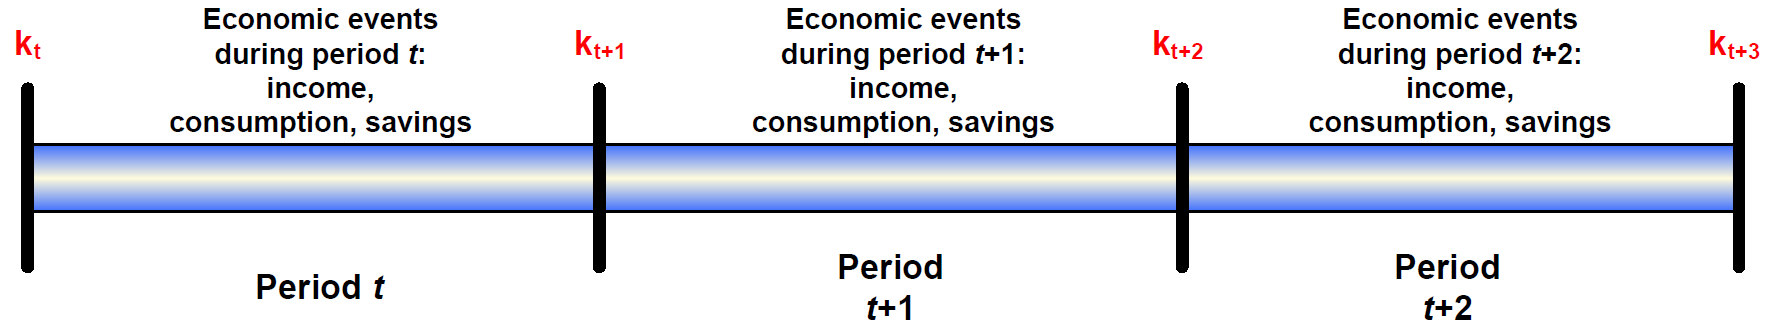
\includegraphics[trim=0 0 0 0,clip,width=1.1\textwidth]{FIGURES/10_Time_cropped}
	}      
	%\subfigure{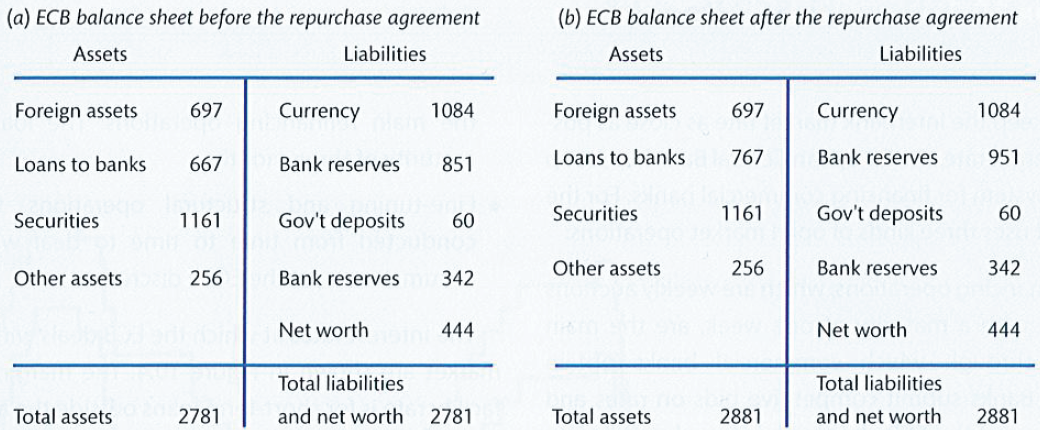
\includegraphics[trim=0 00 0 00,clip,width=0.6\textwidth]{FIGURES/5_CB_balance_sheet_OMO}
	%} 	
	%[trim=left bottom right top
\end{figure}
%\vspace{-2mm}
%\begin{minipage}{0.5\columnwidth}
%\tiny	
%\textbf{Source.} Burda and Wyplosz (2017), Figure 14.1.\\
%\end{minipage}
\end{center}
\end{frame}


\begin{frame}{Law of motion of productivity}
  Productivity has stochastic component, but can also have persistence: \tm{autoregressive process of order 1} (in logs):
  \vfill
  \begin{align*}
	\ln Z_t = \rho \ln Z_{t-1} + \epsilon_t, \quad \epsilon_t \sim \mathcal N(0, \sigma^2_\epsilon) 
  \end{align*}
where $\epsilon$ is the \tm{white noise} component of the autoregressive process -- the \textbf{source of randomness} in $Z_t$ and \textbf{in the model} in general.
  \vfill
  Productivity of period $t$ is observed at beginning of period (or, equivalently, during $t-1$) -- \tr{before the firm hires and installs capital}.
\end{frame}

\begin{frame}{Law of motion of capital}
  Capital lasts for more than one period. It partially depreciates and is increased by \tb{investment}: 
  \vfill
  \begin{align*}
	K_{t+1} &= K_{t} \underbrace{- \delta K_t}_{\text{depreciation}} + I_t \\
	&= (1-\delta) K_t + I_t
  \end{align*}
  \vfill
  Closed economy \rarr investment is financed only with households' \tb{savings}: $$I_t = \Omega_{t+1} - \Omega_t$$
\end{frame}

\begin{frame}{Intertemporal equilibrium: period $t$}
  \tm{Capital market clearing} \\
  \begin{mytemize}
  \item Capital demand from firm's profit maximization: $K_{t+1} = K^d(r_{t+1}, Z_{t+1})$
  \item Capital supply is savings supply: $I_t = \underbrace{\Omega_{t+1} - \Omega_t}_{=G(E_t r_t)}$ 
  \item Combining with law of motion of capital: 
	\begin{equation*}
	  K^d(r_{t+1}, Z_{t+1}) = (1-\delta)K_t + G(E_t r_{t+1})
	\end{equation*}
  \end{mytemize}
\vfill
\tm{Goods-market clearing}
\begin{mytemize}
\item Goods aggregate demand is $C_t+I_t \ \ (= C_t + K_{t+1} - (1-\delta)K_t)$ 
\item Goods aggregate supply is $Y_t$, given by $Z_t f(K_t,L_t)$
\item Goods market clearing
\begin{align*}
  C_t+K_{t+1}-(1-\delta)K_t=Z_t f(K_t,L_t)
\end{align*}
\item[\rarr] \tb{aggregate resource constraint}
\end{mytemize}
\vfill
\tm{Labor market clearing}
\begin{align*}
  L^s(w_t, C_t) = L^d(w_t, Z_t)
\end{align*}
\end{frame}
%---FRAME------------------------------------------------------------------------------
\begin{frame}{States, controls, transversality}

  The economy can be characterized by dynamics of four variables $(Z_t, K_t, C_t, L_t)$ that are divided in two types: 
\begin{mytemize}
\item $Z_t, K_t$ are \tm{state variables} -- depend on the past
\item $C_t, L_t$ are \tm{control} or \tm{jump} variables -- can change instantly depending on \textbf{expectations}
\item State variables have \tm{initial conditions}: $Z_0 (=1), K_0$
\item Control/jump variables need a \tm{transversality condition}: information on where the economy ends up as $t \to \infty$
\begin{align*}
%K_0 = \sum_{s=0}^{\infty} \left( \frac{C_s-w_sL_s-\prod_s}{\prod_{\tau=0}^s(1+r_{\tau}-\delta)}\right)+\underbrace{\lim_{T\rightarrow \infty}\frac{K_{T}}{\prod_{\tau=0}^{T}(1+r_{\tau}-\delta)}}_{\lim=0}
\lim_{T\rightarrow \infty}\frac{K_{T}}{\prod_{\tau=0}^{T}(1+r_{\tau}-\delta)} = 0
\end{align*}
\item Obtained by substituting future incomes in the resource constraints
\end{mytemize}


When transversality condition is satisfied, the resource constraint implies $K_0 = \sum_{s=0}^{\infty} \frac{C_s-w_sL_s-\Pi_s}{\prod_{\tau=0}^s(1+r_{\tau}-\delta)}$ -- initial capital in the economy is equal to \textbf{present discounted value} of all future \textbf{dissavings}.

\end{frame}

\begin{frame}{Dynamic equilibrium: definition}

  A \tb{dynamic equilibrium} is a sequence $\left\{ C_t,L_t, K_{t+1},r_t, w_t\right\}_{t=0}^{\infty}$ that, given $K_0, Z_0$ and the exogenous stochastic process $\ln Z_t = \rho \ln Z_{t-1} + \epsilon_t$, satisfies the following:
\begin{mynumerate}
\item Given $\left\{ r_t,w_t\right\}_{t=0}^{\infty}$, $\left\{ C_t, L_t,K_{t+1}\right\}_{t=0}^{\infty}$ satisfies the sequence of \tm{consumption-savings} optimality conditions, \tm{consumption-labor} optimality conditions, \tm{consumer budget constraints} and the \tm{transversality condition}
  \item Given $\left\{r_t, w_t \right\}_{t=0}^{\infty}$, $\left\{ L_t,K_t\right\}_{t=0}^{\infty}$ satisfy \tm{labor market clearing}: $L^s(w_t, C_t)=L^d(w_t, Z_t)=L_t$ and \tm{capital (asset) market clearing} $G(r_{t})=K^d(r_t, Z_t)=K_t$
\item Goods market clears: $C_t+K_{t+1}-(1-\delta)K_t=Z_t f(K_t,L_t)=Y_t$; 
\end{mynumerate}

\end{frame}
%---FRAME------------------------------------------------------------------------------
\begin{frame}{Dynamic equilibrium: equations}

 A dynamic equilibrium is a sequence $\left\{C_t,L_t,K_{t+1},Z_{t+1}, r_t, w_t \right\}_{t=0}^{\infty}$ that, given $K_0, Z_0$, satisfies
\begin{align*}
  1 =& E_t \left[ {\left( \frac{\beta u'_c(C_{t+1},1-L_{t+1})}{u'_c(C_t,1-L_t)}\right)}(1+r_{t+1})\right] \nonumber \\
%1 =& E_t \left[ \left( \frac{\beta \lambda_{t+1}}{\lambda_t}\right)(1+r_{t+1}-\delta)\right] \nonumber\\
\frac{u'_{1-L}(C_t,1-L_t)}{u'_c(C_t,1-L_t)}=& w_t \nonumber\\
 Z_t f'_L(K_t,L_t) =& w_t \nonumber\\
 Z_t f'_K(K_t,L_t) =& r_t + \delta \nonumber\\
C_t+K_{t+1}=& Z_t f(K_t,L_t) +(1-\delta)K_t\nonumber\\
\ln Z_t =& \rho \ln Z_{t-1} + \epsilon_t \nonumber
\end{align*}
for $t=0,1,2,\dots$, as well as transversality condition as $t \to \infty$
\vfill
\vfill
How do we solve it? First, specify the functions $u(\cdot, \cdot), f(\cdot, \cdot)$. \\ Can we then compute the solution on the board? 
\tr{No!} \ {
\includegraphics[width = 0.04\linewidth]{FIGURES/emoji_scared.png}} \\
\vfill
We can only solve RBC \textbf{numerically} -- on the computer.
\end{frame}

%---FRAME------------------------------------------------------------------------------
%\begin{frame}{Dynamic equilibrium -- prices eliminated}
%
%  A dynamic equilibrium is a sequence $\left\{C_t,L_t,K_{t+1},Z_{t+1} \right\}_{t=0}^{\infty}$ that, given $K_0, Z_0$, satisfies
%\begin{align*}
%  1 =& E_t \left[ {\left( \frac{\beta u'_c(C_{t+1},1-L_{t+1})}{u'_c(C_t,1-L_t)}\right)}(1+Z_{t+1} f'_K(K_{t+1},L_{t+1}))\right] \\
%%1 =& E_t \left[ \left( \frac{\beta \lambda_{t+1}}{\lambda_t}\right)(1+Z_{t+1} f'_K(K_{t+1},L_{t+1})-\delta)\right] \nonumber\\
%\frac{u'_{1-L}(C_t,1-L_t)}{u'_c(C_t,1-L_t)}=& Z_t f'_L(K_t,L_t) \nonumber\\
%C_t+K_{t+1}=& Z_t f(K_t,L_t) +(1-\delta)K_t\nonumber\\
%\ln Z_t =& \rho \ln Z_{t-1} + \epsilon_t \nonumber
%\end{align*}
%for $t=0,1,2,\dots$, as well as transversality condition as $t \to \infty$
%\vfill
%How do we solve it? First, specify the functions $u(\cdot, \cdot), f(\cdot, \cdot)$. \\ Can we then compute the solution on the board? 
%\tr{No!} \ {
\includegraphics[width = 0.04\linewidth]{FIGURES/emoji_scared.png}} \\
%\vfill
%We can only solve RBC \textbf{numerically} -- on the computer.
%\end{frame}
%---FRAME------------------------------------------------------------------------------
%\subsection{Planning Problem}
%%---FRAME------------------------------------------------------------------------------
%\begin{frame}
%\frametitle{Outline}
%\tableofcontents[currentsubsection]
%\end{frame}
%%---FRAME------------------------------------------------------------------------------
%%---FRAME------------------------------------------------------------------------------
%\begin{frame}{Summary: Why Microfoundations?}
%
%\begin{mytemize}
%\small
%\item Consumer preferences
%\item Production technologies
%\begin{mytemize}
%\small
%\item Operated by firms
%\item but industrial organization not specified
%\end{mytemize}
%\item Perfect competition $\leftrightarrow$ can work with Social Planner problem
%\item Next: a quantitative assessment
%\begin{mytemize}
%\item calibration
%\item simulation
%\item comparison with data and IRFs
%\end{mytemize}
%\end{mytemize}
%
%\end{frame}
\section{Solution techniques}
%---FRAME------------------------------------------------------------------------------
\begin{frame}
\frametitle{Outline}
\tableofcontents[currentsection]
\end{frame}
%---FRAME------------------------------------------------------------------------------
\begin{frame}{Numerical solution: Blanchard-Kahn algorithm}

  Once functions $u(\cdot, \cdot), f(\cdot, \cdot)$ chosen, we \textit{can} do a couple of steps without the computer:
\begin{mynumerate}
\item Find formulas for \tb{steady state} values of variables
\item Find some \tb{linearized} from of model equations (e.g. \tb{log-linearized})
\item Obtain the following \tb{matrix form} of the linear model:
  \begin{align*}
	\begin{bmatrix}x^s_{t+1} \\ E_t x^c_{t+1}\end{bmatrix} = A \begin{bmatrix}x^s_{t} \\ x^c_{t}\end{bmatrix} + R \nu_{t+1}
  \end{align*}
  with $x^s_t$ the \tm{vector of state variables}, $x^s_t$ the \tm{vector of control/jump variables}, $\nu_t$ vector of shocks 
\end{mynumerate}
In practice, these 3 steps can be done with computer, too. Next steps are \textit{supposed to be done with the computer}:
\begin{mynumerate}
\item Find eigenvalues and eigenvectors of the $A$ matrix
\item Check that number of \textbf{unstable} eigenvalues (absolute value $\geq 1$) is same as number of control/jump variables (Blanchard-Kahn condition)
\end{mynumerate}

\end{frame}
%---FRAME------------------------------------------------------------------------------
\begin{frame}{Choosing functional forms}

  \begin{mytemize}
\item \textbf{Preferences} -- the $u(\cdot, \cdot)$:
\begin{align*}
  u(\underset{+}{C_t}, \underset{-}{L_t}) = \ln C_t - \chi \frac{L_t^{1+\eta}}{1+\eta},
\end{align*}
where $\eta$ is the inverse of Frisch elasticity of labor supply, $\chi$ the weight of labor disutility in the utility function. Note the it is labor and not leisure that enters the function.
\item \textbf{Production function} -- the $f(\cdot, \cdot)$ -- Cobb-Douglas:
\begin{align*}
  Y_t = Z_t f(K_t, L_t) = Z_t K_t^{\alpha}L_t^{1-\alpha},
\end{align*}
with $\alpha$ the capital share in total income.
\end{mytemize}

\end{frame}
%---FRAME------------------------------------------------------------------------------
\begin{frame}{Equilibrium equations with chosen functions}

\tm{Consumption-savings} condition (Euler equation):
\begin{align*}
  1 =  E_t \left[\frac{\beta C_{t+1}}{C_t}(1+r_{t+1})\right] 
\end{align*}
\vfill
\tm{Consumption-labor} condition:
\begin{align*}
\chi L_t^\eta C_t=w_t 
\end{align*}
\vfill

Firms' \tm{capital and labor demands}: 
  \begin{align*}
	\alpha Z_t K_t^{\alpha-1} L_t^{1-\alpha} &= r_t + \delta\\ (1-\alpha)Z_t K_t^{\alpha}L_t^{-\alpha} &= w_t
\end{align*}

\tm{Resource constraint}:
\begin{align*}
  C_t+K_{t+1}-(1-\delta)K_t= Z_t K_t^\alpha L_t^{1-\alpha} 
\end{align*}
\end{frame}
%---FRAME------------------------------------------------------------------------------
\begin{frame}{Steady state}

  Substitute constant value for all the variables and the null expected value for the random variable $\epsilon$ \rarr a system of equations is obtained:

\begin{align*}
  1 =  \left[\frac{\beta C_{ss}}{C_{ss}}(1+r_{ss})\right] \quad \Rightarrow \quad \frac{1}{\beta} - 1&= r_{ss}  \\
  \chi L_{ss}^\eta C_{ss} &=w_{ss}  \\
  Z_{ss} &= 1 \\
  \alpha (K_{ss}/L_{ss})^{\alpha-1} &= r_{ss} + \delta \\ 
  (1-\alpha)(K_{ss}/L_{ss})^{\alpha} &= w_{ss} \\
  C_{ss} +\delta K_{ss} &= K_{ss}^\alpha L_{ss}^{1-\alpha}  \\
\end{align*}

\end{frame}
%---FRAME------------------------------------------------------------------------------
\begin{frame}{Calibration}

\begin{center}

\begin{tabular}{c c c c c c c c}
\toprule
$\beta$ & $\alpha$ & $\eta$ & $\chi$ & $\delta$ & $\rho$ & $\sigma_\epsilon$ \\ 
\hline 
0.99 & 0.33 & 1 & 8 & 0.025 & 0.8 & 0.01 \\ 
\bottomrule
\end{tabular} 
\end{center}
\vfill
Where do the values come from?
\begin{mytemize}
\item discount factor $\beta$ to yield real \textit{annual} interest rate of $4\%$ \rarr $\beta = 1/(1+r_{ss})=1/(1+0.04/4)\approx 0.99$ (we divide 0.04 by 4 in formula because \alert{model periods are quarters})
\item Cobb-Douglas production function: $\alpha=1/3$ a long-run estimate of capital share in national income
\item Capital depreciation rate is 10\% annually $(\delta=0.1/4=0.025)$
\item $\chi$ is an unobserved parameter that is chosen to match a \tb{target}: $L_{ss} = 0.33$ 
\item $\rho$ can be manipulated to obtain more or less persistent productivity; $\sigma_\epsilon$ for more or less strong shocks
\end{mytemize}

\end{frame}


\begin{frame}{Log-linearization of equations}
  \tr{Log}-\textbf{linearization} -- most widespread \textbf{linearization} technique when done by hand. Practical -- variables become relative deviations from s.s. value. 
  \vfill
  Use  the following substitution for rules for each variable $x_t$: 
  $$x_t = x_{ss} e^{\tilde x_t}, \quad \text{with} \quad \tilde x_t \equiv \ln x_t - \ln x_{ss}$$ 
\vfill
$\tilde x_t$ is a relative \textbf{deviation of $x_t$ from its steady state} (as a share of s.s. value), because $\ln x_t - \ln x_{ss} ~\approx \frac{x_t - x_{ss}}{x_{ss}}$. \\
  \vfill
  Then, use the following approximations:
  \begin{enumerate}
	\item $e^{\tilde x_t} \approx 1 + \tilde x_t$ ($\Leftrightarrow \ \ln (1+\tilde x_t) \approx \tilde x_t$)
	\item $\tilde x_t \tilde y_t \approx 0$  (we are doing a \textbf{first-order} approximation) 
  \end{enumerate}
  \vfill
  There are many tricks that follow from these rules and simplify the process. See, for example, J. Zietz (2006) ``Log-Linearizing Around the Steady State: A Guide with Examples''
\end{frame}

\begin{frame}{Log-linearized model}
  \begin{align*}
	 E_t \left[ \tilde C_{t+1} - \tilde C_{t} - \frac{r_{ss}}{1+r_{ss}}\tilde r_{t+1}\right] &= 0 \\
	  \tilde C_t + \chi \tilde L_t &=  \tilde w_t \\
	  \tilde Z_t + (\alpha -1) \tilde K_t + (1-\alpha) \tilde L_t &= \frac{r_{ss}}{r_{ss}+\delta}\tilde r_t \\
	  \tilde Z_t + \alpha \tilde K_t -\alpha \tilde L_t &= \tilde w_t \\
	  C_{ss} \tilde C_t + K_{ss} (\tilde K_{t+1} - (1-\delta) \tilde K_t) &= K_{ss}^\alpha L_{ss}^{1-\alpha}(\tilde Z_t + \alpha \tilde K_t + (1-\alpha) \tilde L_t) \\
	  \tilde Z_{t+1} &= \rho \tilde Z_t + \epsilon_t
  \end{align*}
  
\end{frame}
\section{Model results}
%---FRAME------------------------------------------------------------------------------
\begin{frame}
\frametitle{Outline}
\tableofcontents[currentsection]
\end{frame}
%---FRAME------------------------------------------------------------------------------
%---FRAME------------------------------------------------------------------------------
\begin{frame}{Stochastic simulation -- an example}

\begin{center}
%{\small
%Figure. 
%}
\vspace{-5mm}
\begin{figure}[h!]
  \subfigure{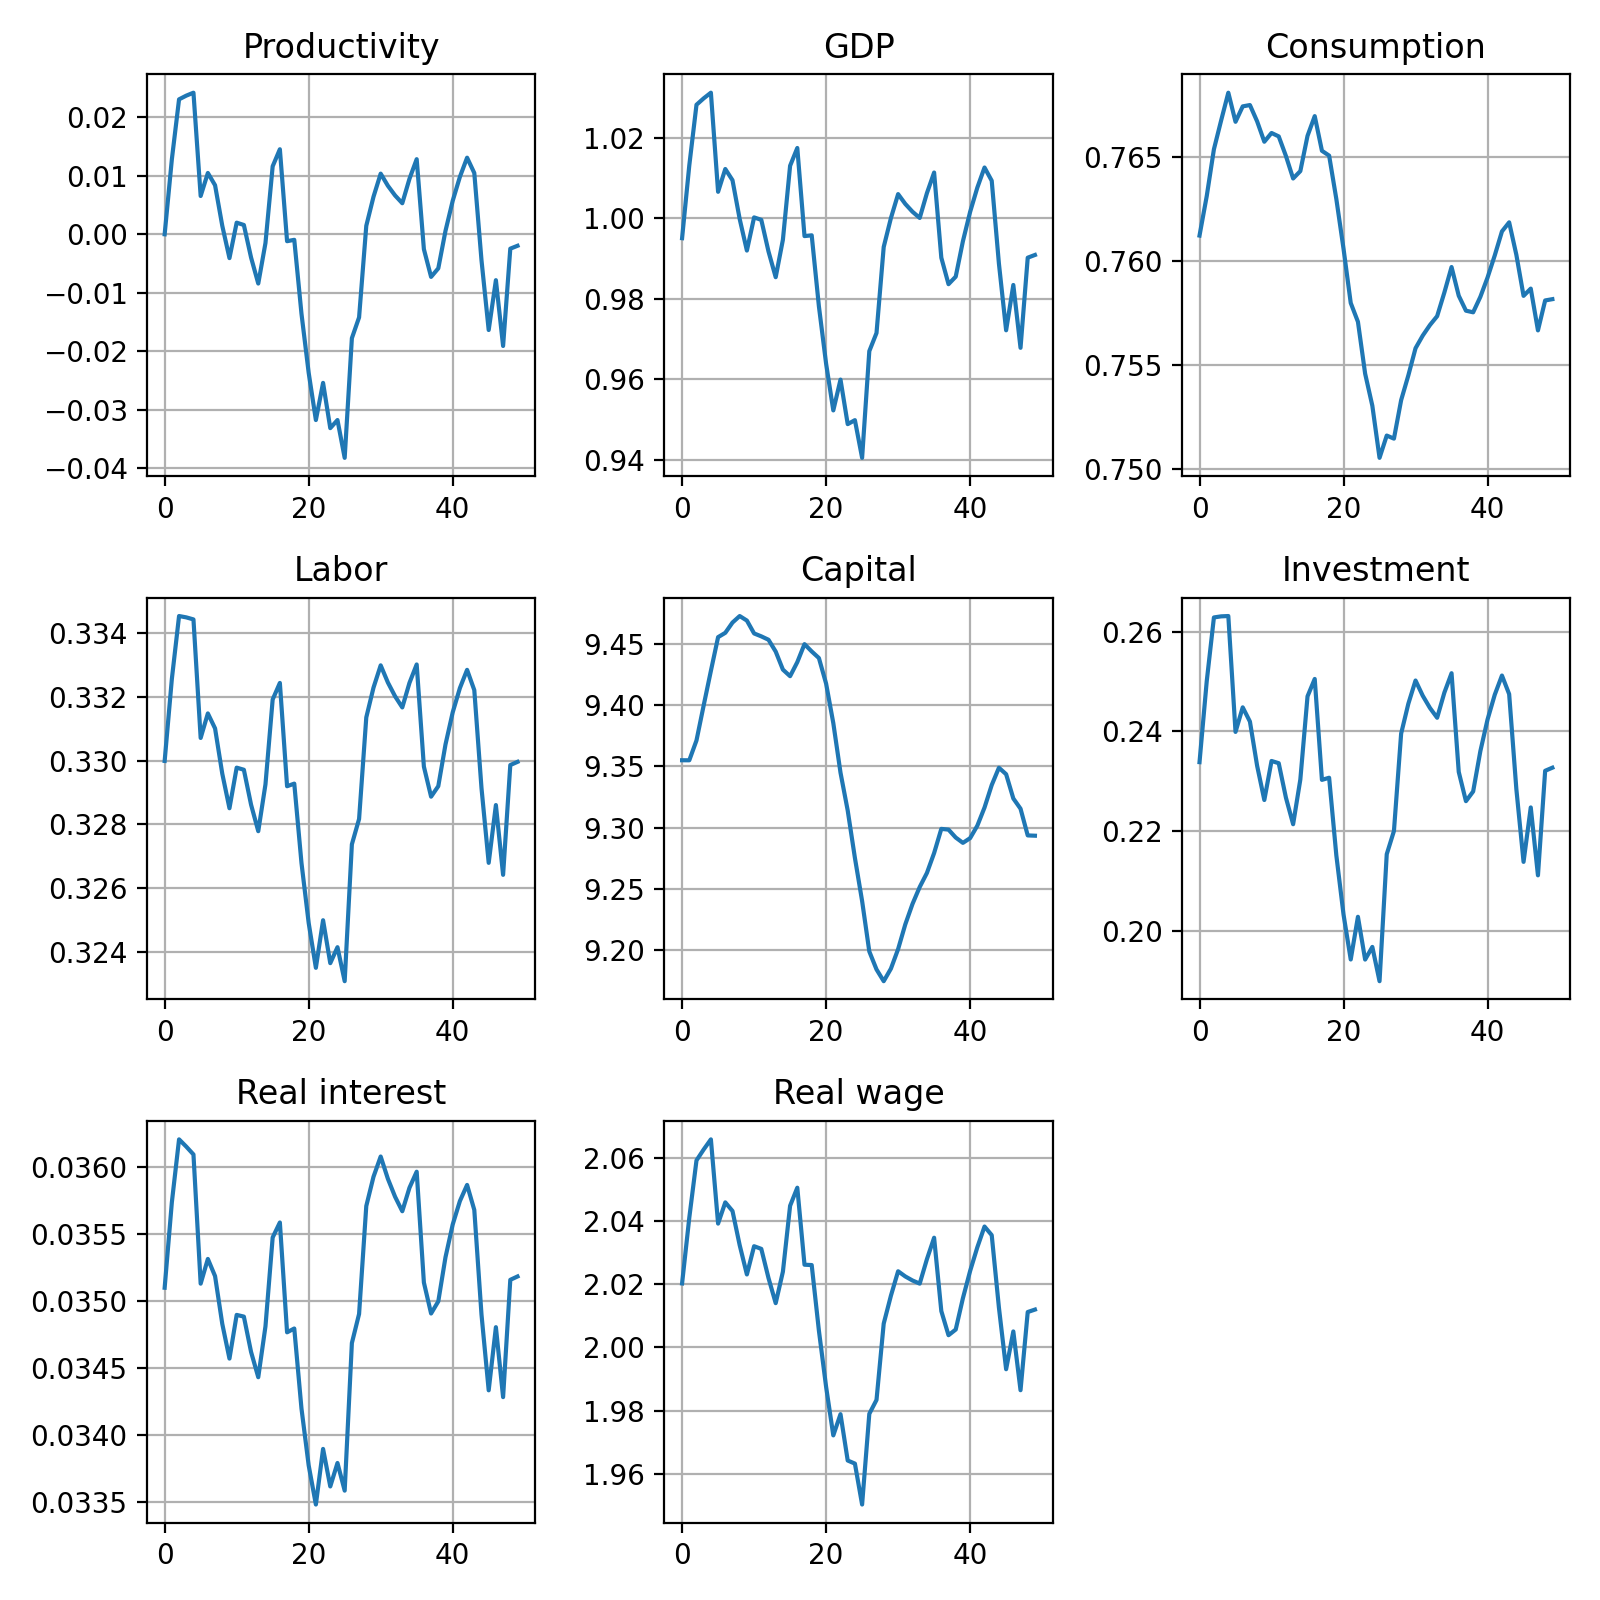
\includegraphics[trim=0 0 0 0,clip,width=0.75\textwidth]{FIGURES/rbc_stochsim8.png}
	}      
	%\subfigure{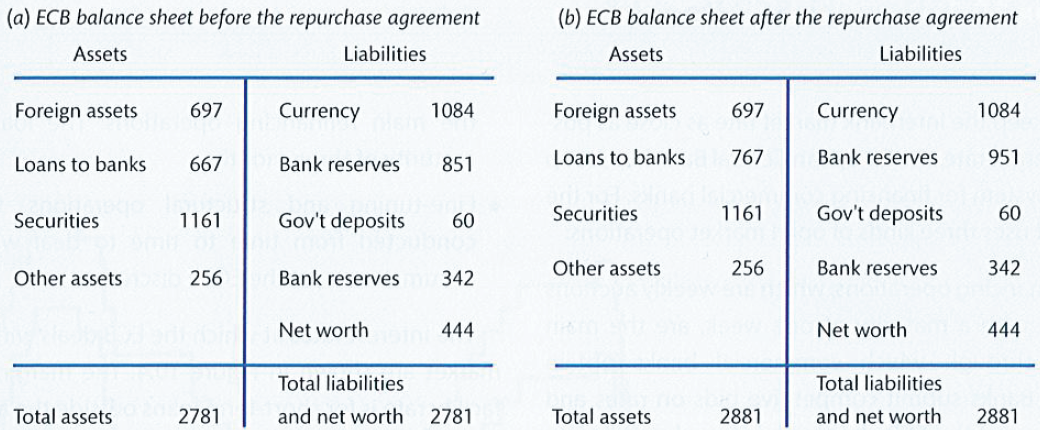
\includegraphics[trim=0 00 0 00,clip,width=0.6\textwidth]{FIGURES/5_CB_balance_sheet_OMO}
	%} 	
	%[trim=left bottom right top
\end{figure}
%\vspace{-2mm}
%\begin{minipage}{0.5\columnwidth}
%\tiny	
%\textbf{Source.} Burda and Wyplosz (2017), Figure 14.1.\\
%\end{minipage}
\end{center}
\vspace{-5mm}
\small
\tr{Attention:} here and henceforth model linearized, not \textbf{log-}linearized by computer \rarr variables in \textbf{levels}, not \textbf{relative deviations} from s.s.
\end{frame}

\begin{frame}{Stochastic simulation -- 1000 examples}

  We simply run the above simulation 1000 times. \textbf{Sequence of shocks is different every time} \rarr dynamics different. Interest and wages not plotted.
\begin{center}
%{\small
%Figure. 
%}
\vspace{-5mm}
\begin{figure}[h!]
  \subfigure{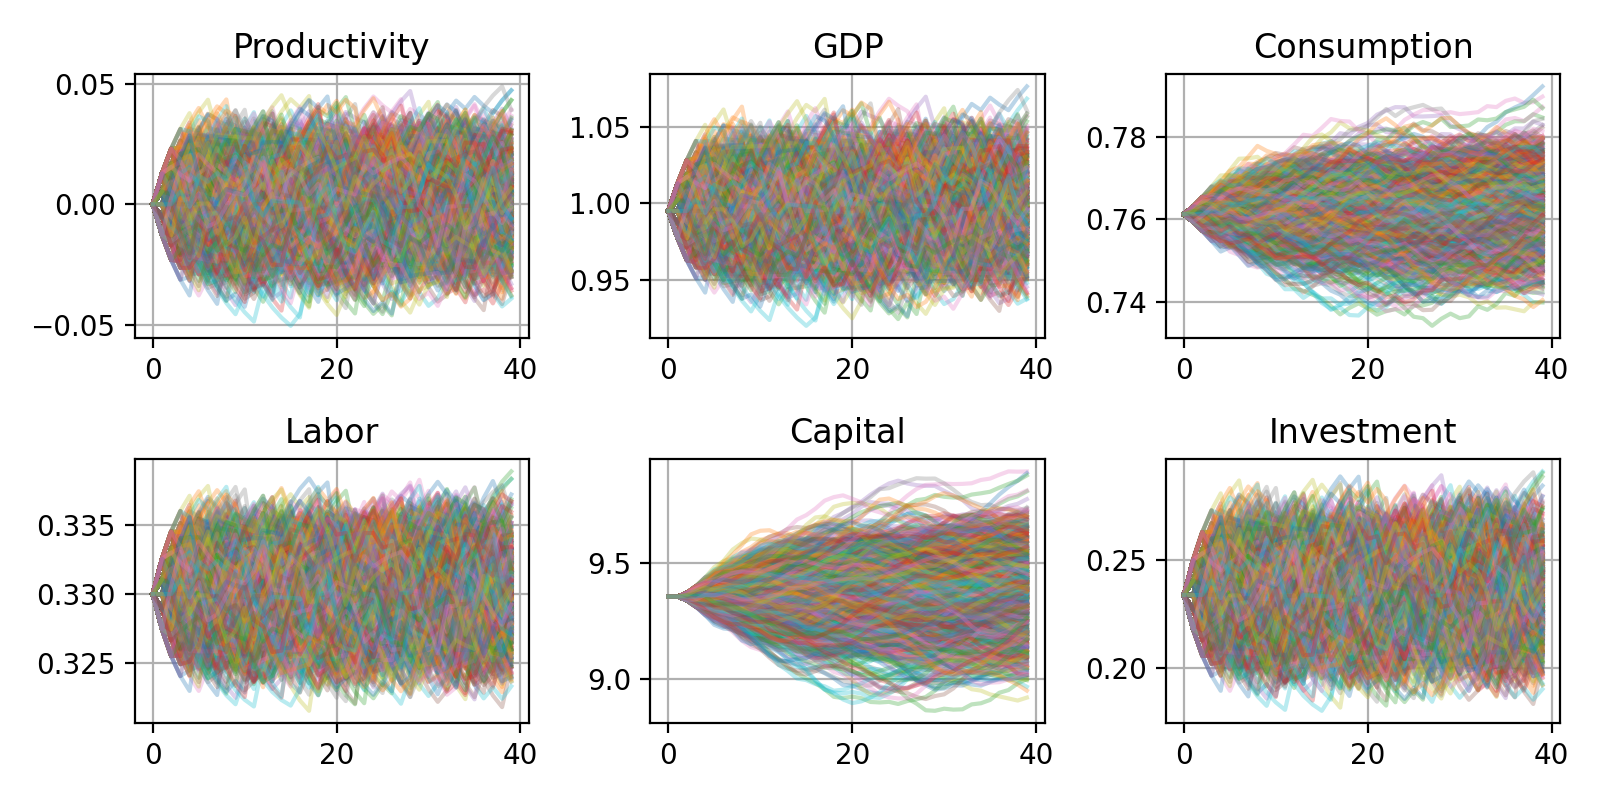
\includegraphics[trim=0 0 0 0,clip,width=0.98\textwidth]{FIGURES/rbc_spaghetti.png}
	}      
	%\subfigure{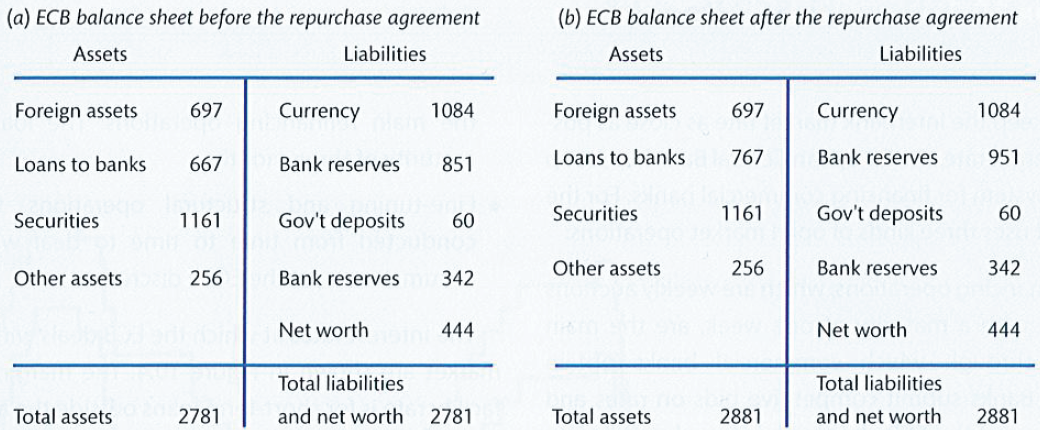
\includegraphics[trim=0 00 0 00,clip,width=0.6\textwidth]{FIGURES/5_CB_balance_sheet_OMO}
	%} 	
	%[trim=left bottom right top
\end{figure}
%\vspace{-2mm}
%\begin{minipage}{0.5\columnwidth}
%\tiny	
%\textbf{Source.} Burda and Wyplosz (2017), Figure 14.1.\\
%\end{minipage}
\end{center}

\end{frame}

\begin{frame}{Model variances vs. empirical variances}
  Compare average standard deviations of 3 variables: GDP, consumption, investment: $\sigma_Y, \sigma_C, \sigma_I$.
  \vfill 
  Model results using 1000 simulations: 
  \begin{mynumerate}
  \item $\sigma_C = 0.15 \sigma_Y$ (\textit{how does it follow form consumer behavior?})
  \item $\sigma_I = 4.5 \sigma_Y$ 
  \end{mynumerate}
  \vfill
  Same statistics in US data (King\&Rebelo(1999) Table 1):
  \begin{mynumerate}
  \item $\sigma_C = 0.74 \sigma_Y$ 
  \item $\sigma_I = 2.9 \sigma_Y$ 
  \end{mynumerate}
  The model exaggerates the difference in variances, but \textbf{reproduces the pattern}: $\sigma_C < \sigma_Y < \sigma_I$ \\
  Easy to improve quantitative performance with more advanced functional forms.


\end{frame}

%---FRAME------------------------------------------------------------------------------
\begin{frame}{Impulse response functions --- Z, Y}

  Transitory productivity shock: $\epsilon$ rises from 0 to $\sigma_\epsilon$ at $t=2$ and is at 0 afterwards:
\begin{center}
%{\small
%Figure. 
%}
\vspace{-5mm}
\begin{figure}[h!]
  \subfigure{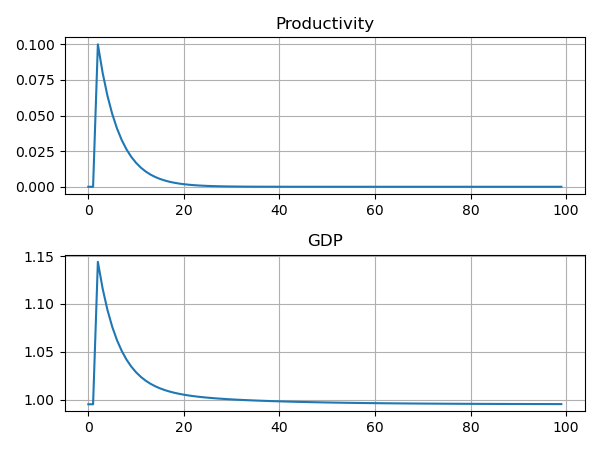
\includegraphics[trim=0 0 0 0,clip,width=0.9\textwidth]{FIGURES/irf_z_y.png}
	}      
	%\subfigure{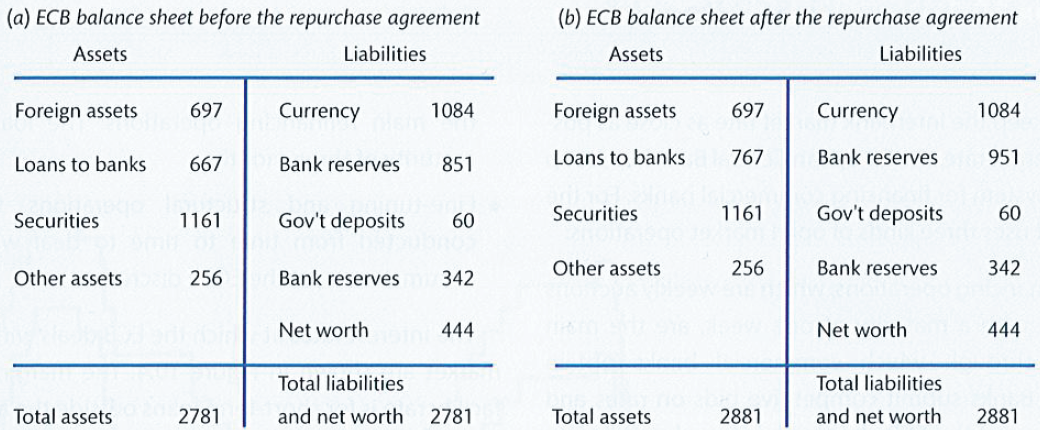
\includegraphics[trim=0 00 0 00,clip,width=0.6\textwidth]{FIGURES/5_CB_balance_sheet_OMO}
	%} 	
	%[trim=left bottom right top
\end{figure}
%\vspace{-2mm}
%\begin{minipage}{0.5\columnwidth}
%\tiny	
%\textbf{Source.} Burda and Wyplosz (2017), Figure 14.1.\\
%\end{minipage}
\end{center}

\end{frame}

\begin{frame}{Impulse response functions --- C, L}

  Transitory productivity shock: $\epsilon$ rises from 0 to $\sigma_\epsilon$ at $t=2$ and is at 0 afterwards:
\begin{center}
%{\small
%Figure. 
%}
\vspace{-5mm}
\begin{figure}[h!]
  \subfigure{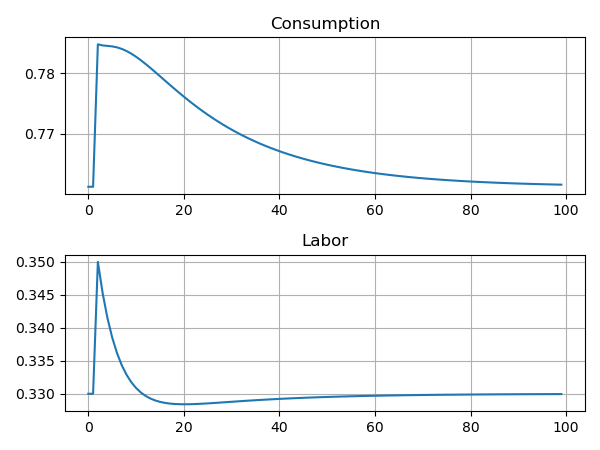
\includegraphics[trim=0 0 0 0,clip,width=0.9\textwidth]{FIGURES/irf_c_l.png}
	}      
	%\subfigure{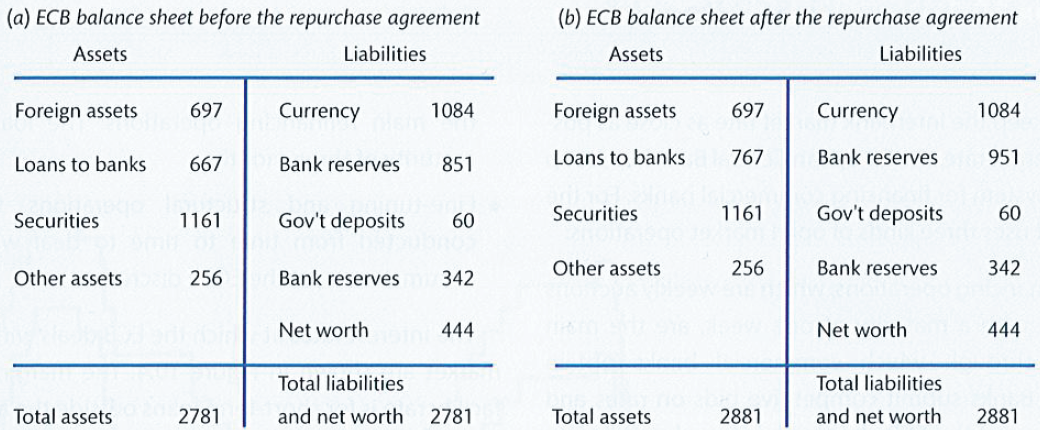
\includegraphics[trim=0 00 0 00,clip,width=0.6\textwidth]{FIGURES/5_CB_balance_sheet_OMO}
	%} 	
	%[trim=left bottom right top
\end{figure}
%\vspace{-2mm}
%\begin{minipage}{0.5\columnwidth}
%\tiny	
%\textbf{Source.} Burda and Wyplosz (2017), Figure 14.1.\\
%\end{minipage}
\end{center}

\end{frame}

\begin{frame}{Impulse response functions --- I, K}

  Transitory productivity shock: $\epsilon$ rises from 0 to $\sigma_\epsilon$ at $t=2$ and is at 0 afterwards:
\begin{center}
%{\small
%Figure. 
%}
\vspace{-5mm}
\begin{figure}[h!]
  \subfigure{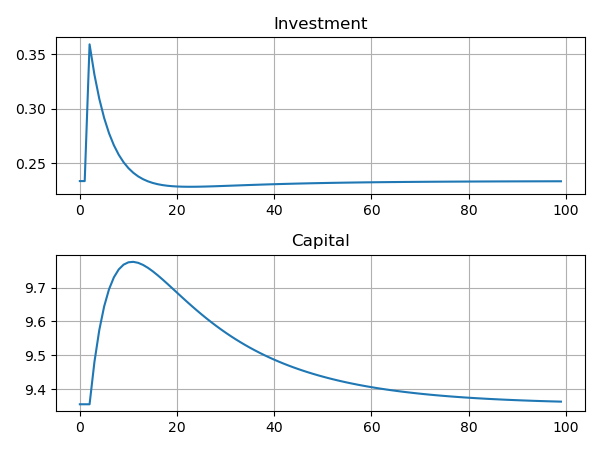
\includegraphics[trim=0 0 0 0,clip,width=0.9\textwidth]{FIGURES/irf_i_k.png}
	}      
	%\subfigure{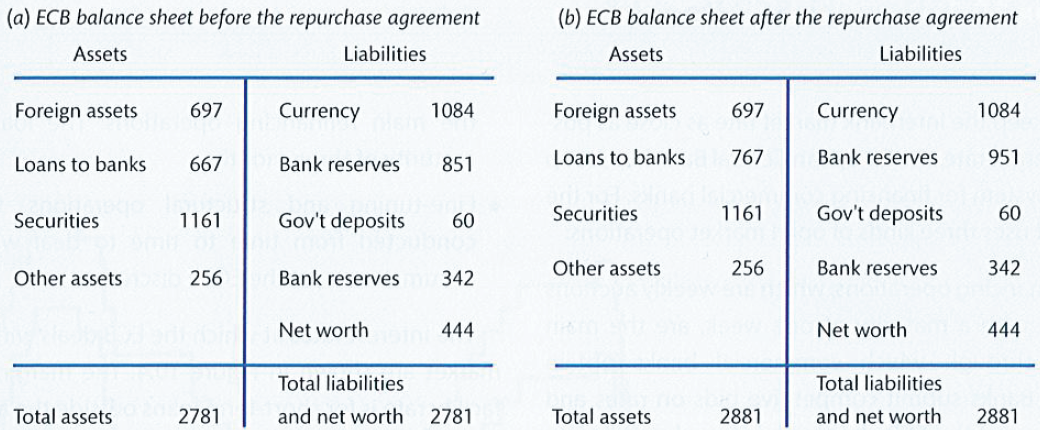
\includegraphics[trim=0 00 0 00,clip,width=0.6\textwidth]{FIGURES/5_CB_balance_sheet_OMO}
	%} 	
	%[trim=left bottom right top
\end{figure}
%\vspace{-2mm}
%\begin{minipage}{0.5\columnwidth}
%\tiny	
%\textbf{Source.} Burda and Wyplosz (2017), Figure 14.1.\\
%\end{minipage}
\end{center}

\end{frame}

\begin{frame}{Transitory vs. permanent productivity shock}

  Transitory shock (blue) -- as before; \\ \textbf{Permanent, anticipated shock} (orange) -- $\epsilon_t > 0$ constant for $t \geq 2$, such that steady-state $Z$ is $\sigma_\epsilon$:
\begin{center}
%{\small
%Figure. 
%}
\vspace{-5mm}
\begin{figure}[h!]
  \subfigure{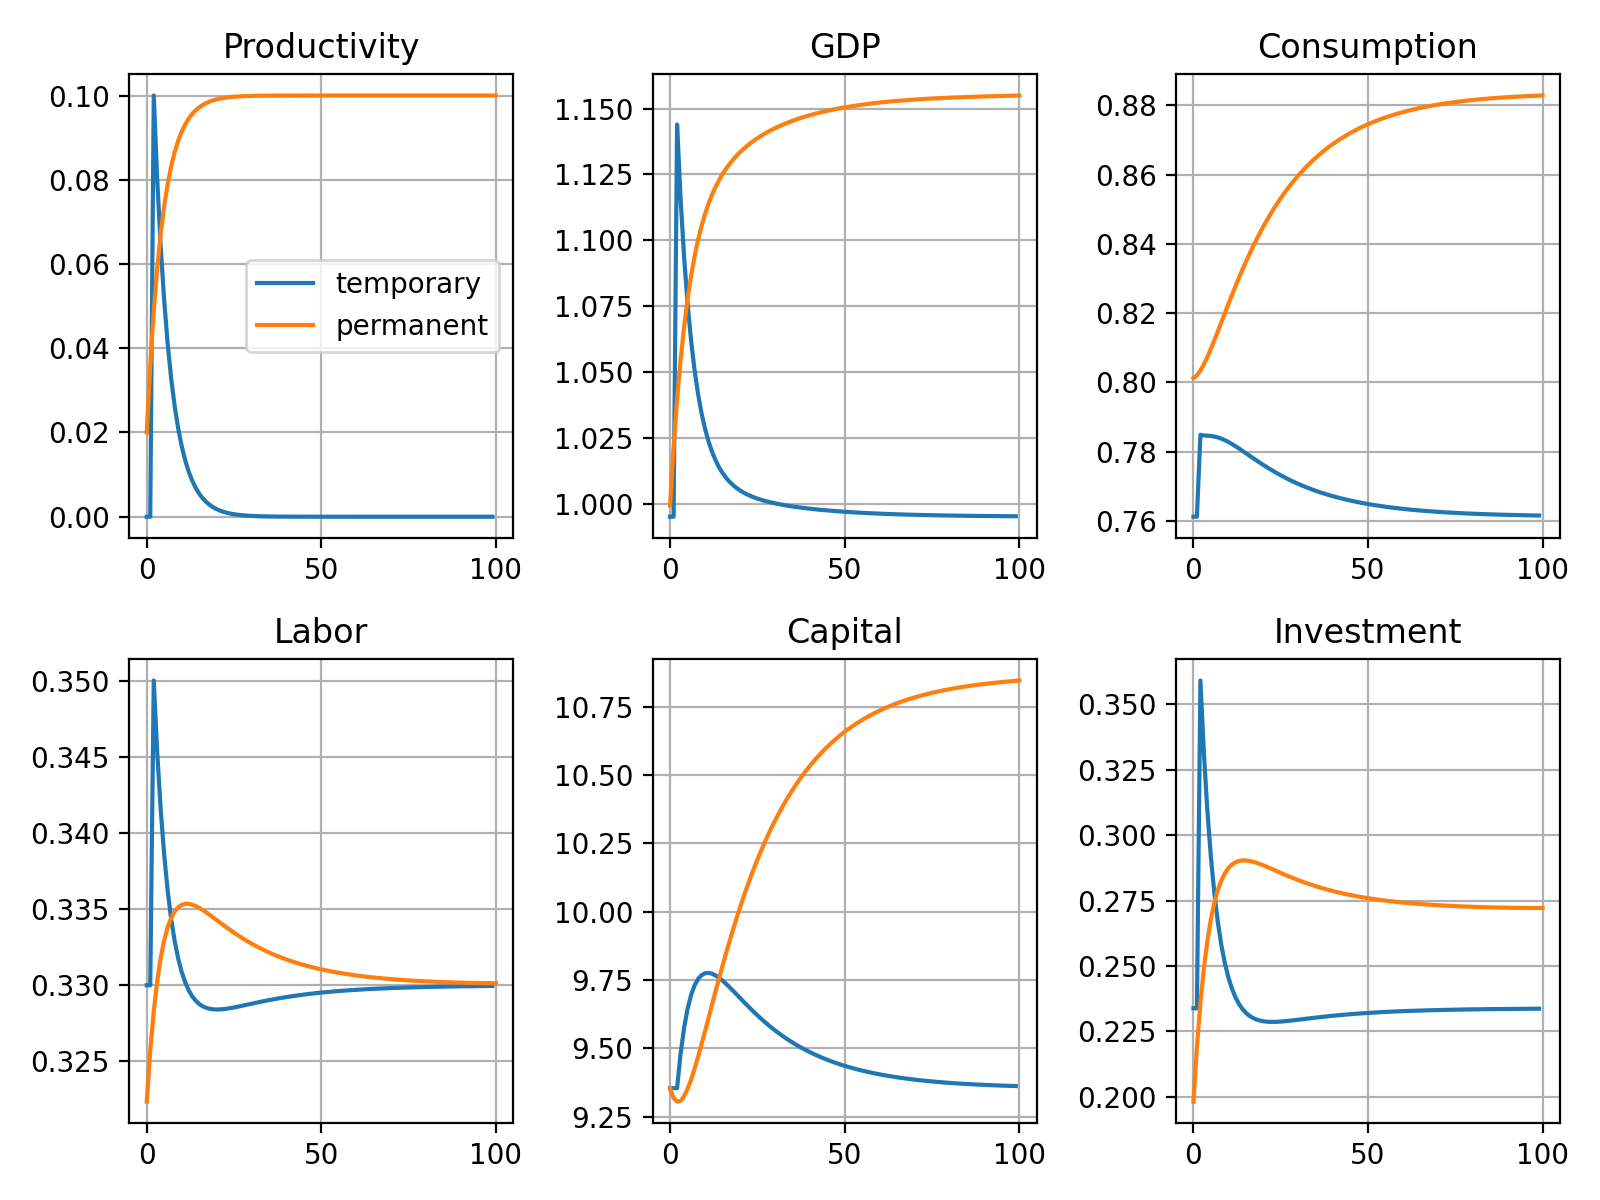
\includegraphics[trim=0 0 0 0,clip,width=0.85\textwidth]{FIGURES/perm_temp_lowsigma.png}
	}      
	%\subfigure{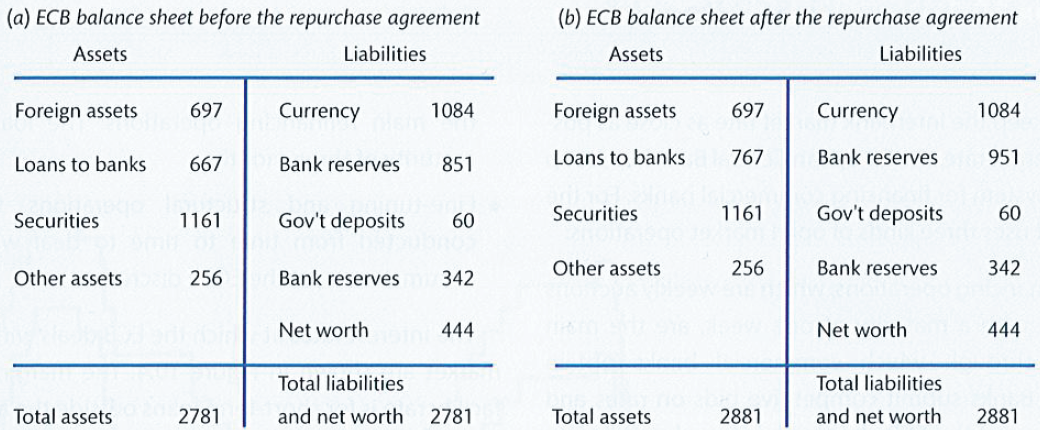
\includegraphics[trim=0 00 0 00,clip,width=0.6\textwidth]{FIGURES/5_CB_balance_sheet_OMO}
	%} 	
	%[trim=left bottom right top
\end{figure}
%\vspace{-2mm}
%\begin{minipage}{0.5\columnwidth}
%\tiny	
%\textbf{Source.} Burda and Wyplosz (2017), Figure 14.1.\\
%\end{minipage}
\end{center}
%
\end{frame}

%%---FRAME------------------------------------------------------------------------------
%%---END------------------------------------------------------------------------------
\end{document}
